\documentclass{beamer}
\usetheme{Madrid} % You can change the theme (e.g., "Berlin", "Copenhagen", "Frankfurt")



% Title, Author, and Date
\title[Wavelet on Integral Equation]{Application of Wavelet on Electromagnetic Integral Equation}
\author[]{Mohammad Mahdi Elyasi}
\institute[Amirkabir University of Techonology]{
    Supervisor: Dr. Moradi \\[1cm] % Professor's Name
    Faculty of Electrical Engineering \\ % Faculty Name
}
\date{\today} % Automatically uses today's date


% Customize the title slide layout
\setbeamertemplate{title page}{
    % Blue strip (Madrid theme)
    \vspace*{-0.5cm} % Adjust vertical spacing
    \begin{beamercolorbox}[wd=\paperwidth,ht=0.4cm,dp=0.2cm,center]{frametitle}
    \end{beamercolorbox}

    % Logo below the strip
    \vspace{0.5cm}
    \centering
    
\includegraphics[width=0.2\textwidth]{amirkabir.png} % Replace with your logo file

    % Title details
    \vspace{0.5cm}
    {\usebeamerfont{title}\inserttitle\par}
    \vspace{0.3cm}
    {\usebeamerfont{author}\insertauthor\par}
    {\usebeamerfont{institute}\insertinstitute\par}
    \vspace{0.3cm}
    {\usebeamerfont{date}\insertdate\par}
}
% Begin Document
\begin{document}


% Title Slide
\begin{frame}
    
    \titlepage
\end{frame}

% Table of Contents Slide
\begin{frame}{Outline}
    \tableofcontents
\end{frame}

% Section 1: Brief Overview
\section{Brief Overview}
\begin{frame}{Brief Overview}
    \begin{itemize}
        \vspace*{-\baselineskip}
        \item Basics of wavelets.
        \item Overview of electromagnetic integral equations.
        \item Applications and results.
    \end{itemize}
\end{frame}

\subsection{Importance of Integral Equations}
\begin{frame}{Importance of Integral Equations}
    \begin{itemize}
        \item Provide a mathematical framework for solving electromagnetic problems.
        \item Convert differential equations into a solvable integral form.
        \item Enable numerical solutions for complex geometries and boundary conditions.
        \[
              f(x) = \lambda \int_a^b K(x, t)\phi(t) \,dt + g(x)
        \]
    \end{itemize}
\end{frame}

\subsection{Motivation of Using Wavelet}
\begin{frame}{Motivation of Using Wavelet}
    \begin{itemize}
        \item Efficient representation of functions and signals.
        \item Localized analysis in both time and frequency domains.
        \item Reduction in computational complexity for solving integral equations.
        
    \end{itemize}
\end{frame}

% Section 2: Wavelet's Overview
\section{Wavelet's Overview}
\subsection{Wavelet Basis}
\begin{frame}{Wavelet Basis}
    \begin{itemize}
        \item Wavelet basis functions provide localized representations of signals.
        \item Constructed through dilation and translation of a mother wavelet.
        \item Enable sparse representation of complex signals.
        \[
             \psi_{j,k}(x) = 2^{j/2} \psi(2^j x - k), \, k \in \mathbb{Z}
        \]
    \end{itemize}
\end{frame}

\subsection{Types of Wavelets}
\begin{frame}{Types of Wavelets}
    \begin{itemize}
        \item Haar wavelets: Simplest wavelets with step-like functions.
        \item Daubechies wavelets: Compactly supported wavelets with various smoothness.
        \item Morlet wavelets: Used for time-frequency analysis.
        \vfill % Push the image to the bottom
        \centering
        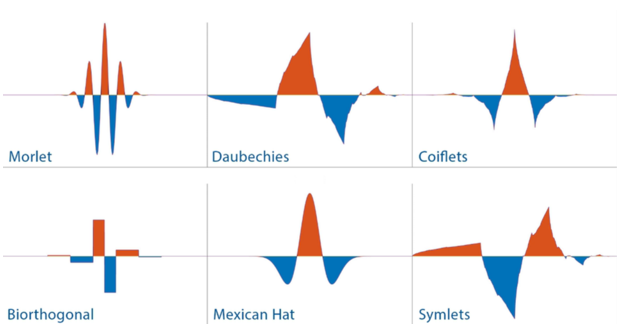
\includegraphics[width=0.8\textwidth]{wavelet.png} % Replace with your image file
        \\[0.2cm] % Add vertical spacing between image and caption
        {\small \textbf Different Wavelets.} % Caption text
        
    \end{itemize}
\end{frame}

\subsection{Advantages of Wavelet}
\begin{frame}{Advantages of Wavelet}
    \begin{itemize}
        \item Multi-resolution analysis for efficient signal representation.
        \item Localized analysis in time and frequency domains.
        \item Reduced computational complexity for large-scale problems.
    \end{itemize}
\end{frame}

% Section 3: Relation between IE and Wavelet
\section{Relation between IE and Wavelet}
\subsection{Types of Integral Equations}
\begin{frame}{Types of Integral Equations}
    \begin{itemize}
        \item Fredholm integral equations: Defined over a fixed range.
        \item Volterra integral equations: Defined over a variable range.
        \item Boundary integral equations: Commonly used in electromagnetic problems.
        \centering
        \[
              f(x) = \int_a^x K(x, t)\phi(t) \,dt + g(x)
        \]
        \\[0.2cm]
        {\small \textbf Volterra IE}
        \[
              f(x) = \lambda \int_a^b K(x, t)\phi(t) \,dt + g(x)
        \]
        \\[0.2cm]
        {\small \textbf Fredholm IE}
    \end{itemize}
\end{frame}

\subsection{Challenges with Traditional Methods}
\begin{frame}{Challenges with Traditional Methods}
    \begin{itemize}
        \item High computational cost for large-scale problems.
        \item Poor convergence for complex geometries.
        \item Difficulty in handling multi-scale behavior.
    \end{itemize}
\end{frame}

\subsection{Why Wavelet Help}
\begin{frame}{Why Wavelet Help}
    \begin{itemize}
        \item Provide sparse representations of integral operators.
        \item Reduce computational complexity with efficient algorithms.
        \item Handle multi-scale behavior effectively.
        \vfil
        \centering
        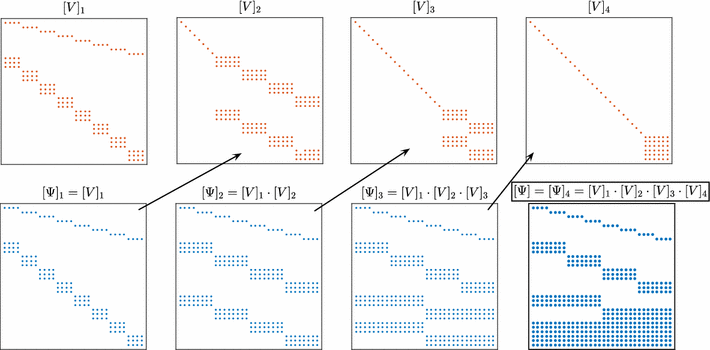
\includegraphics[width=0.8\textwidth]{Example_Sparse_Matrix.png} % Replace with your image file
        \\[0.2cm] % Add vertical spacing between image and caption
        {\small \textbf Example Sparse Matrix} % Caption text
    \end{itemize}
\end{frame}

% Section 4: Applications
\section{Applications}
\subsection{Mathematical Foundation}
\begin{frame}{Mathematical Foundation}
    \begin{itemize}
        \item Underlying mathematical principles of wavelet theory.
        \item Connection between wavelet transforms and integral equations.
        \item Basis for developing efficient computational algorithms.
        \[
              \sum_{j=0}^{n-1} k(\theta_i - \theta_j) \rho(\theta_j) w_j = f(\theta_i), \quad i = 0, 1, \dots, n-1.
        \]
        \[
                \mathbf{K} \boldsymbol{\rho} = \mathbf{f},
        \]
    \end{itemize}
\end{frame}

\subsection{Solved Case}
\begin{frame}{Solved Case}
    \begin{itemize}
        \item Case study of wavelet application in a real-world problem.
        \item Comparison with traditional methods.
        \item Demonstration of improved efficiency and accuracy.\\[0.5cm]
        \vfil
        \centering
        
        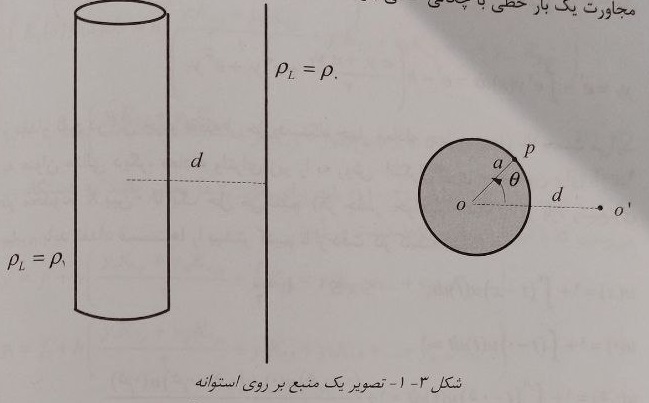
\includegraphics[width=0.5\textwidth, height=0.4\textheight]{Case.jpg} % Replace with your image file
        \\[0.2cm] % Add vertical spacing between image and caption
        {\small \textbf Case Study} % Caption text
    \end{itemize}
\end{frame}

% Section 5: Results
\section{Results}
\begin{frame}{Results}  
    \begin{itemize}
    \item Solved Case for two diferent compilers,"Matlab and Python".\\[0.5cm]
    \end{itemize}
    \centering
    \begin{tabular}{cc}
        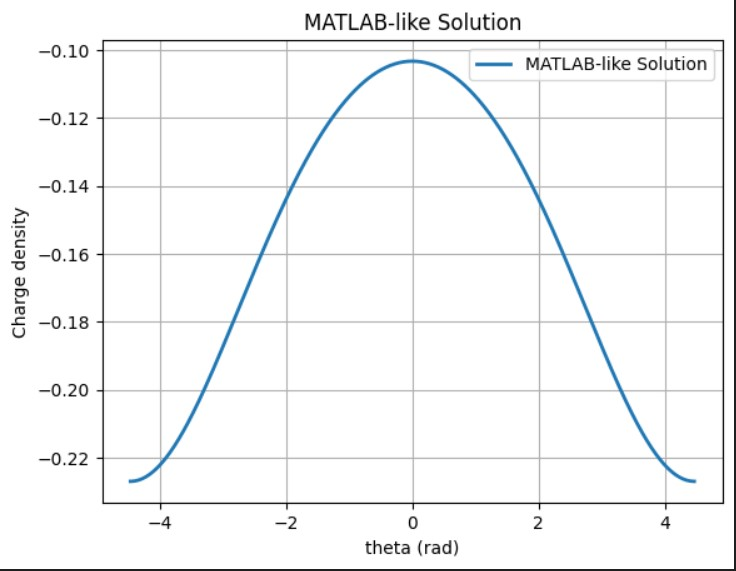
\includegraphics[width=0.45\textwidth]{1.jpg} & 
        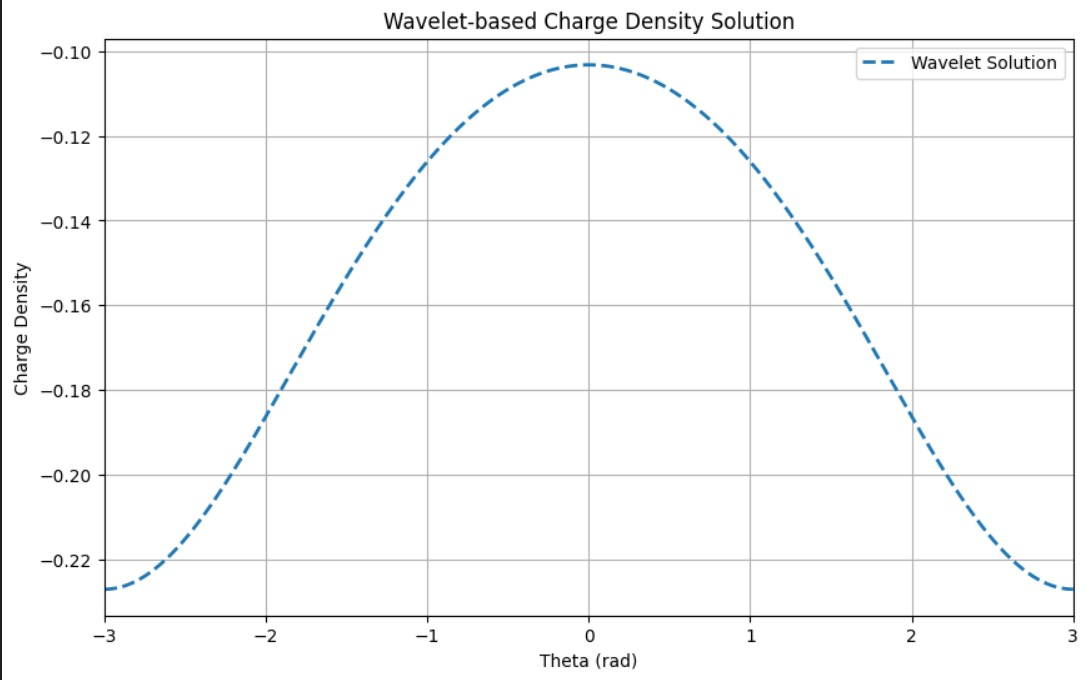
\includegraphics[width=0.45\textwidth]{2.jpg} \\
        {\scriptsize MATLAB-like Solution} & {\scriptsize Wavelet-based Charge Density Solution} \\
        
    \end{tabular}
    
\end{frame}

\begin{frame}{Plots}
        \begin{itemize}
        \item Extraction of Coefficient with Multi-Resolution method.\\[0.5cm]
        \end{itemize}
    \begin{columns}[T]
        \column{0.5\textwidth}
        \centering
        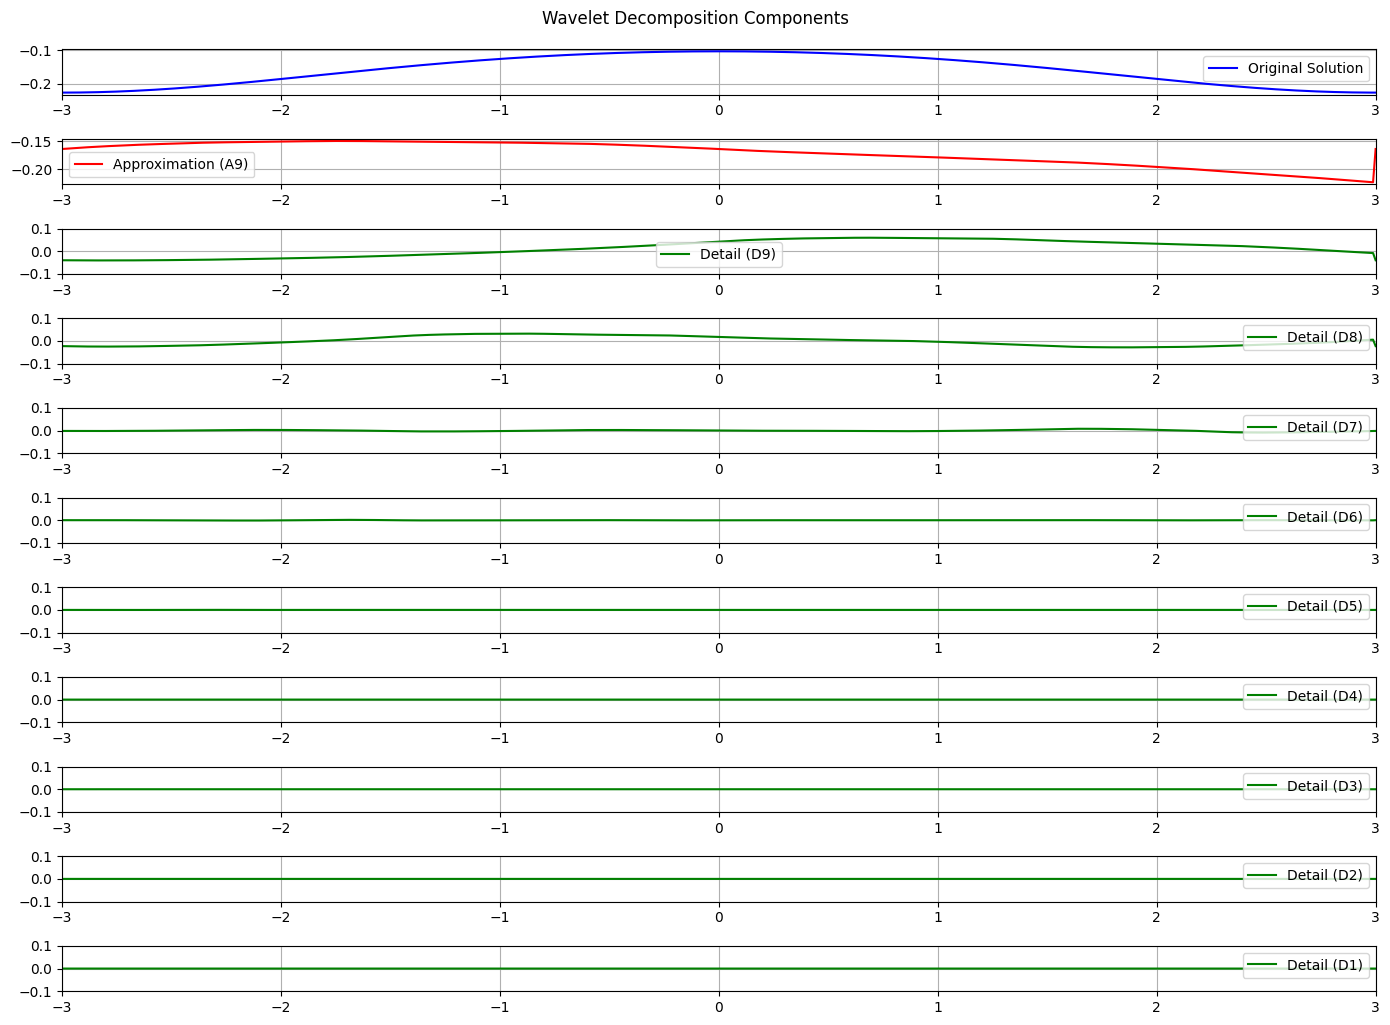
\includegraphics[width=\textwidth]{3.png} \\[0.2cm] % Replace with your image file
        {\scriptsize Detailed and Approximation} % Optional: Add caption
        \column{0.5\textwidth}
        \centering
        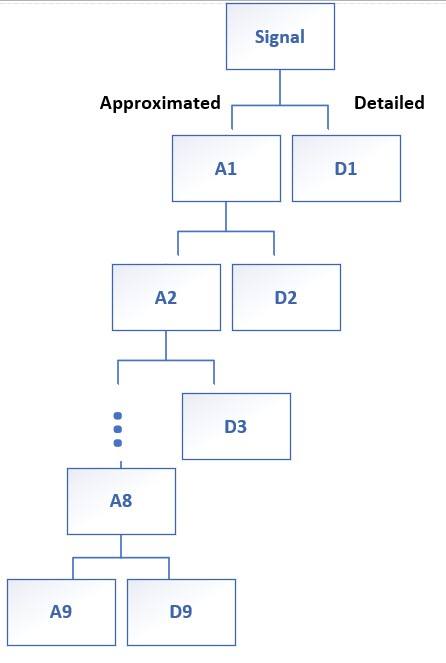
\includegraphics[width=\textwidth, height=0.6\textheight]{Tree graph.jpg} \\[0.2cm] % Replace with your image file
        {\scriptsize Tree Graph} % Optional: Add caption
        
    \end{columns}

\end{frame}

% Section 6: Conclusion
\section{Conclusion}
\begin{frame}{Conclusion}
    \begin{itemize}
        \vspace*{-\baselineskip}
        \item Benefits of wavelets for electromagnetic integral equations.
        \item Wavelet or other methods.
    \end{itemize}
\end{frame}

% Section 7: References
\section{References}
\begin{frame}{References}
    \begin{itemize}
        \item [1] G.Moradi, Advanced Engineering Mathematics,AmirKabir University Of Technology,
        2012 .
        \item [2] I. Daubechies, Ten Lectures on Wavelets, Society for Industrial and Applied Math
       ematics, 1992.
        \item [3] Github link,Application of Wavelet on EFIE at https://github.com/
        MohammadMahdiElyasi/Application-of-Wavelet-in-Elctromagnetic-Integral-Equation.
    \end{itemize}
\end{frame}

% Section 8: Outro
\begin{frame}{Outro}
    \centering
    {\Large \textbf{Thank you for your attention!}} \vspace{1cm} % Ensures proper centering
    \vfill % Pushes the logo to the bottom
    
\includegraphics[width=0.2\textwidth]{amirkabir.png} % Replace with your logo file
\end{frame}

\end{document}